% =========================================================================
%  SafrMrtah — AI Travel Intelligence Platform
%  Project report and user guide
%  Author: Mohamed Makrani — Data Scientist & AI Developer
%  Compile with XeLaTeX (two passes):  xelatex SafrMrtah_Report.tex
% =========================================================================
\documentclass[11pt,a4paper]{article}

% ---------- Page and fonts -----------------------------------------------
\usepackage[a4paper,top=24mm,bottom=24mm,left=24mm,right=24mm,headheight=14pt]{geometry}
\usepackage{fontspec}
\setmainfont{Barlow}[
  Path=fonts/,
  UprightFont=barlow-latin-400-normal.ttf,
  BoldFont=barlow-latin-600-normal.ttf,
  ItalicFont=barlow-latin-400-normal.ttf,
  ItalicFeatures={FakeSlant=0.18},
  BoldItalicFont=barlow-latin-600-normal.ttf,
  BoldItalicFeatures={FakeSlant=0.18}]
\newfontfamily\figures{BarlowSC}[
  Path=fonts/,
  UprightFont=barlow-semi-condensed-latin-600-normal.ttf,
  Numbers=Monospaced]
\newfontfamily\heavy{BarlowBold}[Path=fonts/, UprightFont=barlow-latin-700-normal.ttf]
\setmonofont{DejaVu Sans Mono}[Scale=0.84]
\linespread{1.12}

% ---------- Colour (AviationStack palette, as used in the app) -------------
\usepackage{xcolor}
\definecolor{ink}{HTML}{2F313A}
\definecolor{inkdeep}{HTML}{26282F}
\definecolor{slate}{HTML}{27344A}
\definecolor{slatechart}{HTML}{283F59}
\definecolor{muted}{HTML}{6A7C93}
\definecolor{rule}{HTML}{E3E5E8}
\definecolor{paper}{HTML}{F1F2F5}
\definecolor{brand}{HTML}{2EBC4F}
\definecolor{accent}{HTML}{1A7F33}
\definecolor{tint}{HTML}{E9F7ED}
\definecolor{infotint}{HTML}{EBF1FA}
\definecolor{amber}{HTML}{F79009}
\definecolor{ambertint}{HTML}{FFF6E9}
\definecolor{bad}{HTML}{D92D20}

% ---------- Packages ------------------------------------------------------
\usepackage{graphicx}
\usepackage{booktabs,tabularx,array}
\usepackage{enumitem}
\usepackage[most]{tcolorbox}
\usepackage{titlesec}
\usepackage{fancyhdr}
\usepackage{tikz}
\usetikzlibrary{positioning,arrows.meta,fit,backgrounds,calc,shapes.geometric,svg.path,decorations.markings}

% Contact details (used on the cover and in the sign-off)
\newcommand{\linkedinurl}{https://www.linkedin.com/in/mohamed-makrani-b9bb0028b/}
\newcommand{\emailaddr}{makranimohamed46@gmail.com}
\newcommand{\contactline}{%
  \href{\linkedinurl}{\color{accent}\bfseries LinkedIn}%
  \qquad
  \href{mailto:\emailaddr}{\color{accent}\bfseries Email}}

% Line icons drawn from SVG paths (adapted from Lucide, ISC licence).
% svg.path works in pt, so icons are flipped and centred with transforms.
\tikzset{
  plane icon/.pic={
    \fill[ink] (0,0) circle (17pt);
    \begin{scope}[rotate=-45,scale=1.25,yscale=-1,shift={(-12pt,-12pt)}]
      \draw[white,solid,line width=1.5pt,line cap=round,line join=round]
        svg {M17.8 19.2 16 11l3.5-3.5C21 6 21.5 4 21 3c-1-.5-3 0-4.5 1.5L13 8 4.8 6.2c-.5-.1-.9.1-1.1.5l-.3.5c-.2.5-.1 1 .3 1.3L9 12l-2 3H4l-1 1 3 2 2 3 1-1v-3l3-2 3.5 5.3c.3.4.8.5 1.3.3l.5-.2c.4-.3.6-.7.5-1.2z};
    \end{scope}},
  pin icon/.pic={
    \begin{scope}[scale=1.25,yscale=-1,shift={(-12pt,-22pt)}]
      \draw[brand,solid,fill=ink,line width=1.5pt,line cap=round,line join=round]
        svg {M20 10c0 4.993-5.539 10.193-7.399 11.799a1 1 0 0 1-1.202 0C9.539 20.193 4 14.993 4 10a8 8 0 0 1 16 0};
      \draw[brand,solid,line width=1.5pt] (12pt,10pt) circle (3pt);
    \end{scope}}
}

\usepackage[hidelinks]{hyperref}
\usepackage{microtype}

\hypersetup{pdftitle={SafrMrtah - Project report and user guide},
            pdfauthor={Mohamed Makrani}}

% ---------- Headings ------------------------------------------------------
\titleformat{\section}{\color{slate}\heavy\Large}{\color{accent}\thesection}{0.8em}{}
\titlespacing*{\section}{0pt}{20pt}{8pt}
\titleformat{\subsection}{\color{slate}\bfseries\large}{\color{muted}\thesubsection}{0.7em}{}
\titlespacing*{\subsection}{0pt}{14pt}{5pt}
\titleformat{\subsubsection}{\color{slate}\bfseries}{}{0em}{}

\setlength{\parindent}{0pt}
\setlength{\parskip}{6pt}
\setlist{itemsep=2pt,topsep=3pt,leftmargin=1.4em}
\setlist[itemize]{label={\color{accent}\textbullet}}

% ---------- Header / footer -----------------------------------------------
\pagestyle{fancy}
\fancyhf{}
\fancyhead[L]{\small\color{muted}SafrMrtah \,|\, Project report and user guide}
\fancyhead[R]{\small\color{muted}Mohamed Makrani}
\fancyfoot[R]{\small\color{muted}\thepage}
\renewcommand{\headrulewidth}{0.4pt}
\renewcommand{\headrule}{\color{rule}\hrule width\headwidth height\headrulewidth}

% ---------- Boxes ---------------------------------------------------------
\newtcolorbox{keybox}[1][]{enhanced,colback=tint,colframe=tint,boxrule=0pt,
  borderline west={3pt}{0pt}{brand},arc=2pt,left=10pt,right=10pt,top=7pt,bottom=7pt,#1}
\newtcolorbox{notebox}[1][]{enhanced,colback=ambertint,colframe=ambertint,boxrule=0pt,
  borderline west={3pt}{0pt}{amber},arc=2pt,left=10pt,right=10pt,top=7pt,bottom=7pt,#1}
\newtcolorbox{shot}{enhanced,colback=white,colframe=rule,boxrule=0.6pt,arc=3pt,
  left=0pt,right=0pt,top=0pt,bottom=0pt}

\newcommand{\shotfig}[3]{%
  \begin{figure}[htbp]\centering
  \begin{shot}\includegraphics[width=\linewidth]{#1}\end{shot}
  \caption{#2}\label{#3}\end{figure}}
\usepackage{caption}
\captionsetup{font={small,color=muted},labelfont={bf,color=slate},justification=raggedright,singlelinecheck=false}

\newcolumntype{L}{>{\raggedright\arraybackslash}X}
\renewcommand{\arraystretch}{1.3}
\newcommand{\code}[1]{\texttt{\color{slate}#1}}

% =========================================================================
\begin{document}

% ---------------------------- Title page ---------------------------------
\begin{titlepage}
\newgeometry{margin=0mm}
\thispagestyle{empty}
\begin{tikzpicture}[remember picture,overlay]
  % charcoal band
  \fill[ink] (current page.north west) rectangle ([yshift=-158mm]current page.north east);
  % flight path: departure dot -- flown (solid) -- plane -- to go (dashed) -- destination pin
  \coordinate (dep) at ([xshift=26mm,yshift=-112mm]current page.north west);
  \coordinate (pln) at ([xshift=118mm,yshift=-112mm]current page.north west);
  \coordinate (dst) at ([xshift=-28mm,yshift=-112mm]current page.north east);
  \draw[brand,line width=1.4pt] (dep) -- (pln);
  \draw[brand!40,line width=1.4pt,dash pattern=on 6pt off 6pt] (pln) -- (dst);
  \fill[brand] (dep) circle (3pt);
  \draw[brand!45,line width=0.9pt] (dep) circle (6.5pt);
  \pic at (pln) {plane icon};
  \pic at (dst) {pin icon};
  % perforation
  \draw[white!25!ink,dash pattern=on 4pt off 4pt,line width=1pt] ([yshift=-158mm]current page.north west) -- ([yshift=-158mm]current page.north east);
  % brand
  \node[anchor=north west,text=white,font=\heavy\fontsize{15}{15}\selectfont] at ([xshift=24mm,yshift=-22mm]current page.north west) {SafrMrtah};
  \node[anchor=north east,text=white!60!ink,font=\small] at ([xshift=-24mm,yshift=-23mm]current page.north east) {Version 2.0 \quad November 2026};
  \node[anchor=north west,text width=150mm,text=white,font=\heavy\fontsize{30}{36}\selectfont] at ([xshift=24mm,yshift=-38mm]current page.north west)
    {AI travel intelligence platform};
  \node[anchor=north west,text width=150mm,text=white!70!ink,font=\Large] at ([xshift=24mm,yshift=-62mm]current page.north west)
    {Project report and user guide};
  \node[anchor=north west,text=white,font=\heavy\fontsize{20}{24}\selectfont] at ([xshift=24mm,yshift=-126mm]current page.north west) {Plan your next destination.};
\end{tikzpicture}

\vspace*{172mm}
\hspace*{24mm}\begin{minipage}{162mm}
{\color{muted}\small Prepared by}\\[2mm]
{\heavy\fontsize{24}{28}\selectfont\color{slate} Mohamed Makrani}\\[2mm]
{\Large\color{accent} Data Scientist \& AI Developer}\\[4mm]
{\small\contactline}

\vspace{11mm}
{\color{muted}\small Technologies}\\[1.5mm]
{\color{slate}\large FastAPI \;\textbullet\; LangGraph \;\textbullet\; Model Context Protocol (MCP) \;\textbullet\; Groq LLM\\[1mm]
AviationStack \;\textbullet\; Tavily \;\textbullet\; OpenWeather \;\textbullet\; PostgreSQL \;\textbullet\; Docker \;\textbullet\; Render}

\vspace{14mm}
\begin{minipage}[t]{80mm}
{\color{muted}\small What this document covers}\\[1.5mm]
\color{slate}What SafrMrtah is and who it is for, how to use it, how the agents work together, the system architecture, and how to run and deploy it.
\end{minipage}\hfill
\begin{minipage}[t]{70mm}
{\color{muted}\small Date}\\[1.5mm]
{\color{slate}22 November 2026}
\end{minipage}
\end{minipage}
\restoregeometry
\end{titlepage}

% ---------------------------- Contents -----------------------------------
\setcounter{page}{2}
{\hypersetup{linkcolor=slate}\tableofcontents}
\clearpage

% =========================================================================
\section{Executive summary}

\textbf{SafrMrtah} turns a trip described in everyday language into a reviewed, day-by-day travel plan. A traveller writes, for example, \emph{``5 days from Dhaka to Dubai with flights, hotels, weather and sightseeing''}. A \emph{supervisor} AI agent reads the request, decides which specialist agents are needed, and coordinates them: flights, hotels, weather, costs and the itinerary. The result is a draft that the traveller checks and approves, or asks to change, before it becomes final.

\begin{keybox}
\textbf{In one sentence:} SafrMrtah is a multi-agent AI travel planner that combines live aviation, search and weather data with a large language model, and keeps a human in control of the final plan.
\end{keybox}

Three principles guide the product:

\begin{itemize}
  \item \textbf{Trust before polish.} The interface shows only information the agents actually returned. When something is missing it says ``Not available'' instead of inventing a price, a flight or a forecast.
  \item \textbf{A person has the last word.} Every plan pauses for human approval. The traveller can approve it or describe changes, and the agents revise the draft.
  \item \textbf{Plans are kept.} Each trip is stored in a database under its own identifier, so it survives a browser refresh, a server restart or a move to another computer.
\end{itemize}

% =========================================================================
\section{The product, without the technology}

\subsection{The problem}
Planning a trip means jumping between airline sites, hotel listings, weather apps and a spreadsheet for the budget, then stitching it all into a daily plan. The information is scattered, it changes, and it is easy to plan a beach day during a heatwave or to miss that the flight budget alone is already gone.

\subsection{What SafrMrtah does for the traveller}
\begin{itemize}
  \item \textbf{One request, one plan.} The traveller describes the trip once, in their own words.
  \item \textbf{Everything in one place.} Flights, hotels, weather, costs and the daily plan each have their own page, all about the same trip.
  \item \textbf{Live data where it matters.} Airports and schedules come from AviationStack, current weather and a 5-day forecast from OpenWeather, hotel options from a live web search.
  \item \textbf{Honest numbers.} Fares and costs are labelled as estimates; nothing is presented as a live price.
  \item \textbf{Several trips side by side.} Every request becomes a trip in ``Your trips'', and the traveller can switch between them at any time.
  \item \textbf{Something to keep.} The full plan can be copied or downloaded as a PDF.
\end{itemize}

\subsection{Who it is for}
\begin{tabularx}{\linewidth}{@{}>{\leavevmode\color{slate}\bfseries}p{38mm}L@{}}
\toprule
Travellers & People planning a holiday or a business trip who want a complete draft in minutes and stay in control of the final version. \\
Travel advisers & Professionals who prepare itineraries for clients and want a fast first draft to review and adjust. \\
Teams and recruiters & A working demonstration of agentic AI: supervisor routing, tool use through MCP, guardrails and human-in-the-loop approval. \\
\bottomrule
\end{tabularx}

\subsection{Design choices}
The interface borrows from airports: a boarding-pass card shows the route with its airport codes, and the colours follow the AviationStack visual identity (charcoal, green and slate). Text is written for travellers rather than engineers, and technical details such as agent names, thread identifiers or model calls stay out of sight. The layout adapts to phones, keyboard focus is visible, and motion is reduced when the device asks for it.

% =========================================================================
\section{How to use SafrMrtah}

\subsection{Sign in}
On a deployed server, the browser asks for a username and password the first time (the owner sets them; the default username is \code{admin}). On your own computer the site opens directly.

\subsection{Plan a trip}
\begin{enumerate}[leftmargin=1.6em]
  \item Open \textbf{Overview}. Under ``Where are you going?'', describe the trip: where from, where to, how long, and what matters (flights, hotel level, budget, activities).
  \item Or pick an example under \emph{Try}, such as ``Dhaka to Dubai''.
  \item Click \textbf{Plan this trip} (or press \code{Ctrl+Enter}). A progress bar shows the plan is being prepared; everything appears at once when it is ready.
\end{enumerate}

\shotfig{img/plan.png}{Starting a new trip.}{fig:plan}

\begin{keybox}
\textbf{Tips for a good request.} Name the departure and destination cities, the number of days, and what you want covered. ``7 days in Japan from Bangladesh, flights, mid-range hotels, under 2 lakhs'' works better than ``Japan trip''. If you leave out a topic, for example flights, that part is simply not planned.
\end{keybox}

\subsection{Read the overview}
The overview shows the boarding pass for the route (airport codes, trip length, typical fare and flight time), key figures (destination, where to stay, weather now, estimated total), the day-by-day preview, estimated costs, and \emph{What we checked}, a short list showing which parts of the trip were looked at.

\shotfig{img/overview.png}{The overview of a draft trip (sample data).}{fig:overview}

\subsection{Approve or request changes}
Every new plan is a \textbf{draft}. At the top of the page, \emph{Your plan is ready to check} offers two choices:
\begin{itemize}
  \item \textbf{Approve plan} keeps the draft as the final plan. The status becomes \emph{Approved}.
  \item \textbf{Request changes} needs a short note under ``Anything to change?'', for example ``cheaper hotel, and keep day 3 free''. The plan is rewritten with your note and the status becomes \emph{Updated}.
\end{itemize}

\begin{figure}[htbp]\centering
\begin{shot}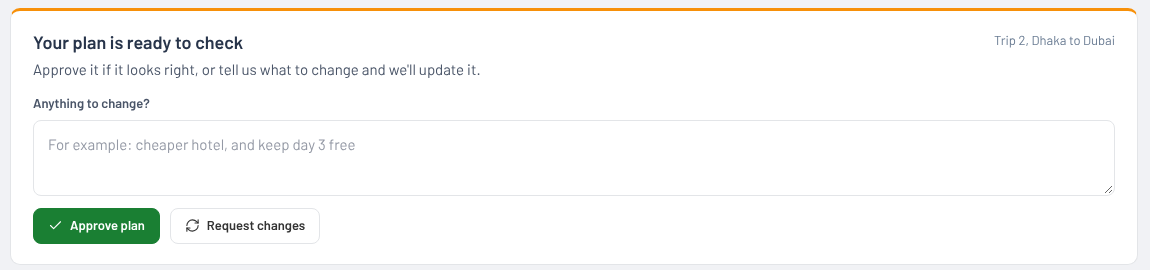
\includegraphics[width=\linewidth]{img/approval.png}\end{shot}
\caption{The approval box. On the Flights, Hotels, Weather and Budget pages it shrinks to a single line.}
\end{figure}

\subsection{Explore each part of the trip}
The left-hand menu opens one page per topic. Each page only shows that topic for the selected trip; if your request did not ask about it, the page says so.

\begin{tabularx}{\linewidth}{@{}>{\leavevmode\color{slate}\bfseries}p{28mm}L@{}}
\toprule
Overview & Boarding pass, key figures, day-by-day preview, costs, what was checked. \\
Flights & Route and airport names, airlines, stops, flight time, typical fare, flight options and advice. \\
Hotels & Recommended area and hotel, nightly price range, total accommodation cost, shortlist, links to the places online. \\
Weather & Current temperature, feels-like, humidity, wind, the next 5 days as a chart, what to pack, best time to be outside. \\
Budget & Estimated total, whether it fits your budget, cost per category with a bar chart, every cost line, risks and ways to save. \\
Itinerary & A card for each day with morning, afternoon, evening and transport, plus a summary and practical tips. \\
Full plan & The complete plan as written, with \textbf{Copy text} and \textbf{Download PDF}. \\
\bottomrule
\end{tabularx}

\begin{figure}[htbp]\centering
\begin{minipage}[t]{0.49\linewidth}\begin{shot}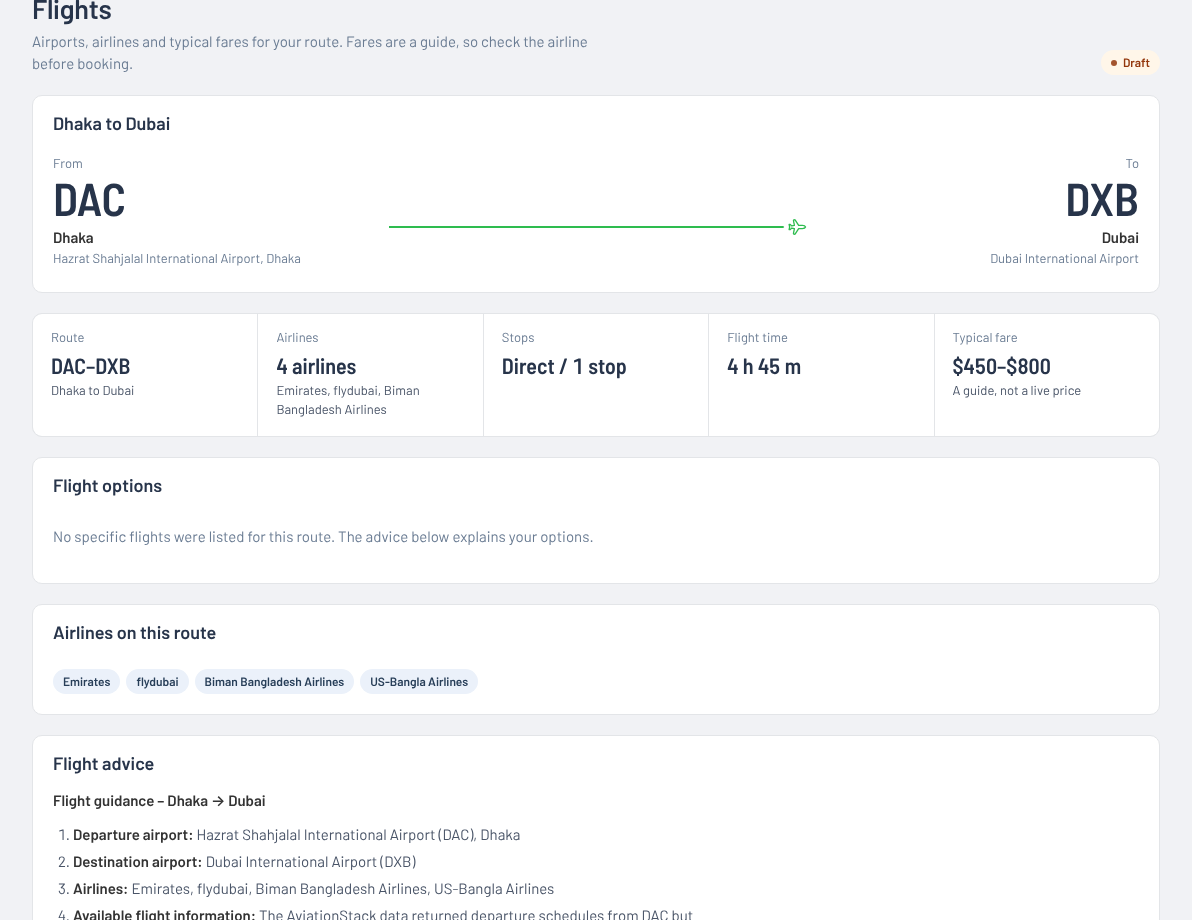
\includegraphics[width=\linewidth]{img/flights.png}\end{shot}\end{minipage}\hfill
\begin{minipage}[t]{0.49\linewidth}\begin{shot}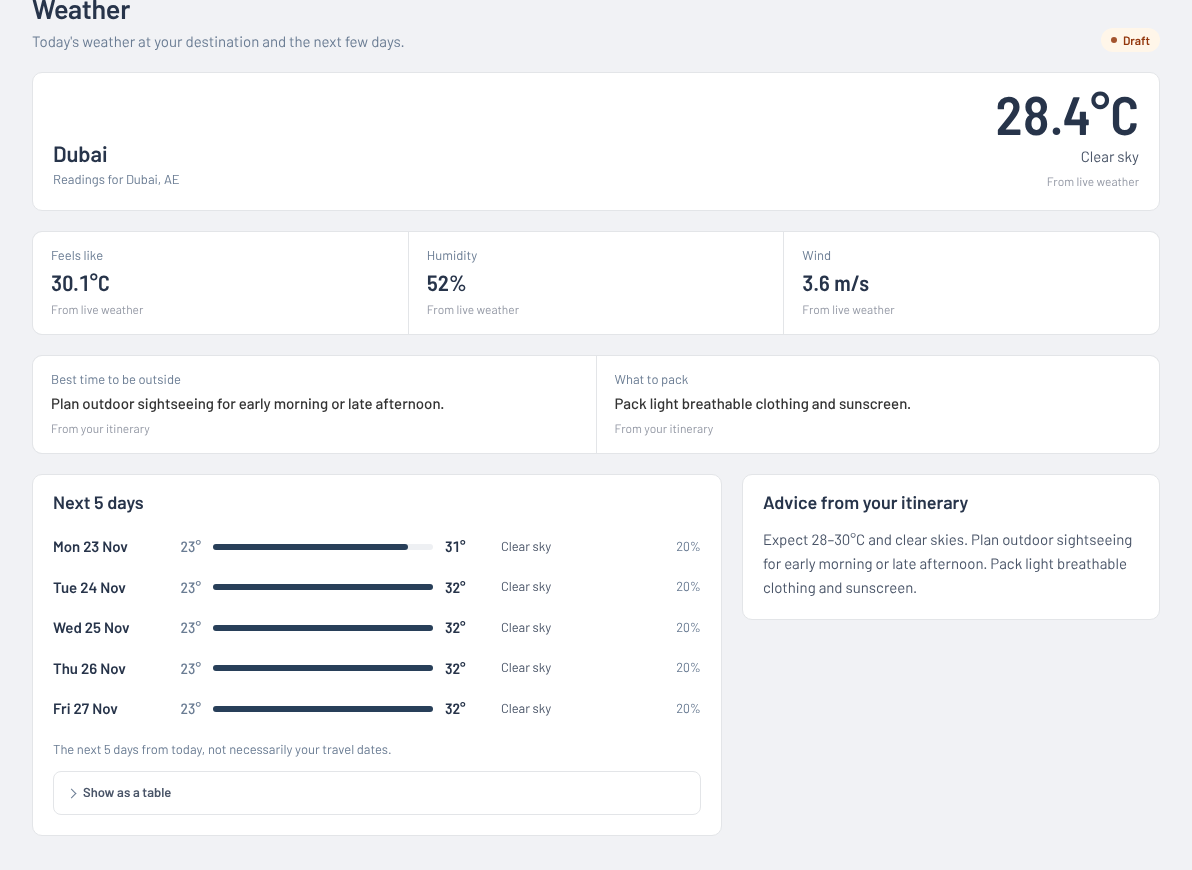
\includegraphics[width=\linewidth]{img/weather.png}\end{shot}\end{minipage}
\caption{Flights and Weather pages (sample data).}
\end{figure}

\begin{figure}[htbp]\centering
\begin{minipage}[t]{0.49\linewidth}\begin{shot}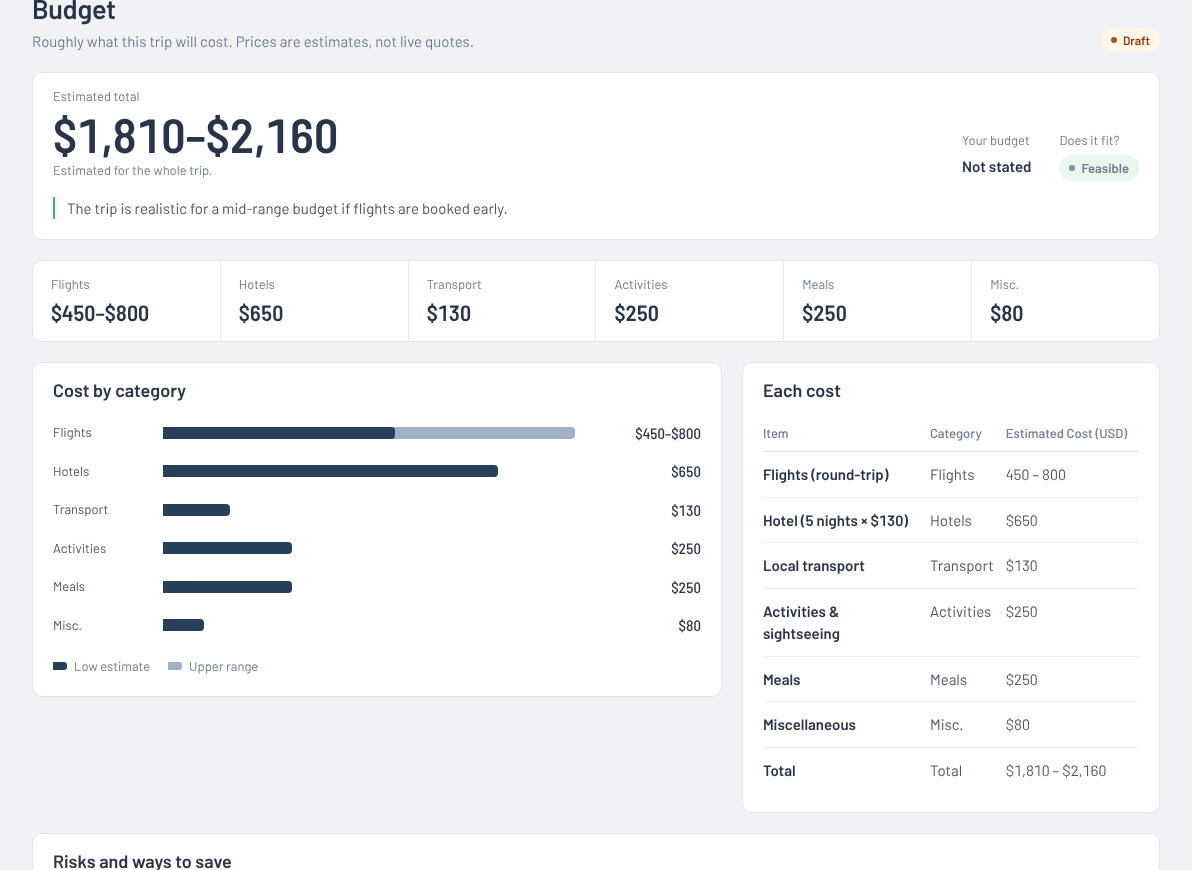
\includegraphics[width=\linewidth]{img/budget.png}\end{shot}\end{minipage}\hfill
\begin{minipage}[t]{0.49\linewidth}\begin{shot}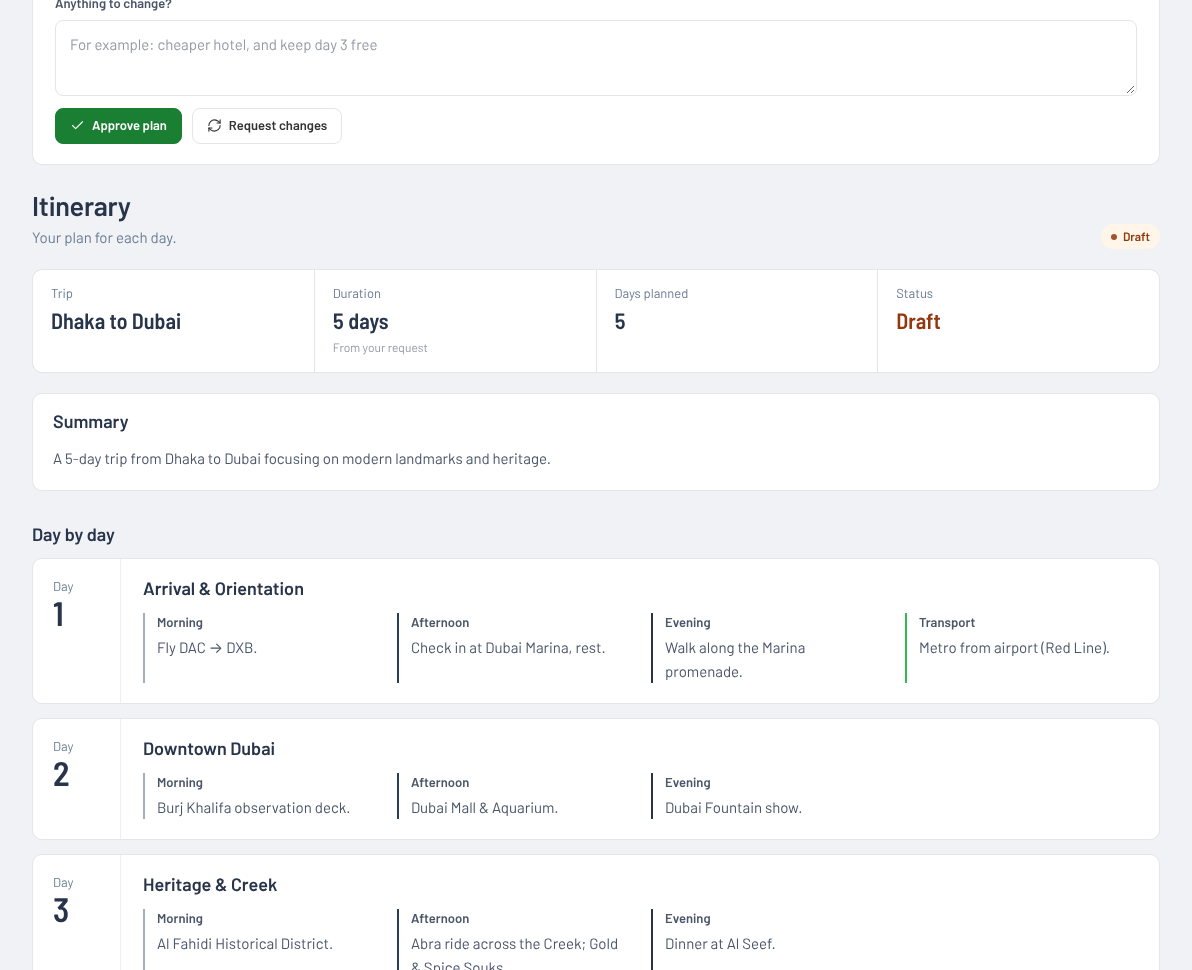
\includegraphics[width=\linewidth]{img/itinerary.png}\end{shot}\end{minipage}
\caption{Budget and Itinerary pages (sample data).}
\end{figure}

\subsection{Manage several trips}
Each request creates a new trip under \textbf{Your trips} in the sidebar (Trip 1, Trip 2, \dots), with its route, length, date and status. Click a trip to open it; click \textbf{New} or \textbf{New trip} to plan another. A draft can wait: you can approve it later.

\subsection{Reading the statuses}
\begin{tabularx}{\linewidth}{@{}>{\bfseries}p{28mm}L@{}}
\toprule
\leavevmode\color{amber}Draft & The plan is ready and waiting for your approval. \\
\leavevmode\color{accent}Approved & You approved the plan; it is final. \\
\leavevmode\color{slatechart}Updated & You asked for changes and the plan was rewritten. \\
\leavevmode\color{bad}Not planned & The request was not about travel, so nothing was planned. \\
\bottomrule
\end{tabularx}

\begin{notebox}
\textbf{Good to know.} Fares and costs are estimates, not quotes. The weather forecast covers the next five days from today, not necessarily your travel dates. Always confirm prices and schedules with the airline or hotel before booking.
\end{notebox}

% =========================================================================
\section{Technology}

\subsection{Technology stack}
\begin{tabularx}{\linewidth}{@{}>{\leavevmode\color{slate}\bfseries}p{34mm}>{\raggedright\arraybackslash}p{44mm}L@{}}
\toprule
Layer & Technology & Role \\
\midrule
Web server & FastAPI, Uvicorn & API endpoints, serves the interface, optional password protection \\
Orchestration & LangGraph & Supervisor routing, agent sequence, human-approval pause \\
Language model & Groq (\code{openai/gpt-oss-120b}) & Guardrail, routing, flight analysis, budget, itinerary, revisions \\
Tool access & Model Context Protocol (MCP), \code{langchain-mcp-adapters} & Uniform access to external data tools \\
Flight data & AviationStack MCP server & Airport schedules (departures, arrivals) \\
Web search & Tavily MCP server & Airport code lookup and hotel search \\
Weather & Custom weather MCP server (OpenWeather) & Current conditions and 5-day forecast; remote over Streamable HTTP \\
Persistence & PostgreSQL, LangGraph checkpointer & Every step of every trip saved under its thread ID \\
Interface & HTML, CSS, JavaScript; Marked.js; html2pdf.js & Dashboard, Markdown rendering, PDF export \\
Delivery & Docker, Render & Container image and hosting \\
\bottomrule
\end{tabularx}

\subsection{Architecture}
Figure~\ref{fig:arch} shows how the parts connect. The browser talks only to the FastAPI server. The server runs the LangGraph workflow, which calls the language model on Groq and reaches external data through MCP servers. Every step is checkpointed in PostgreSQL.

\begin{figure}[htbp]\centering
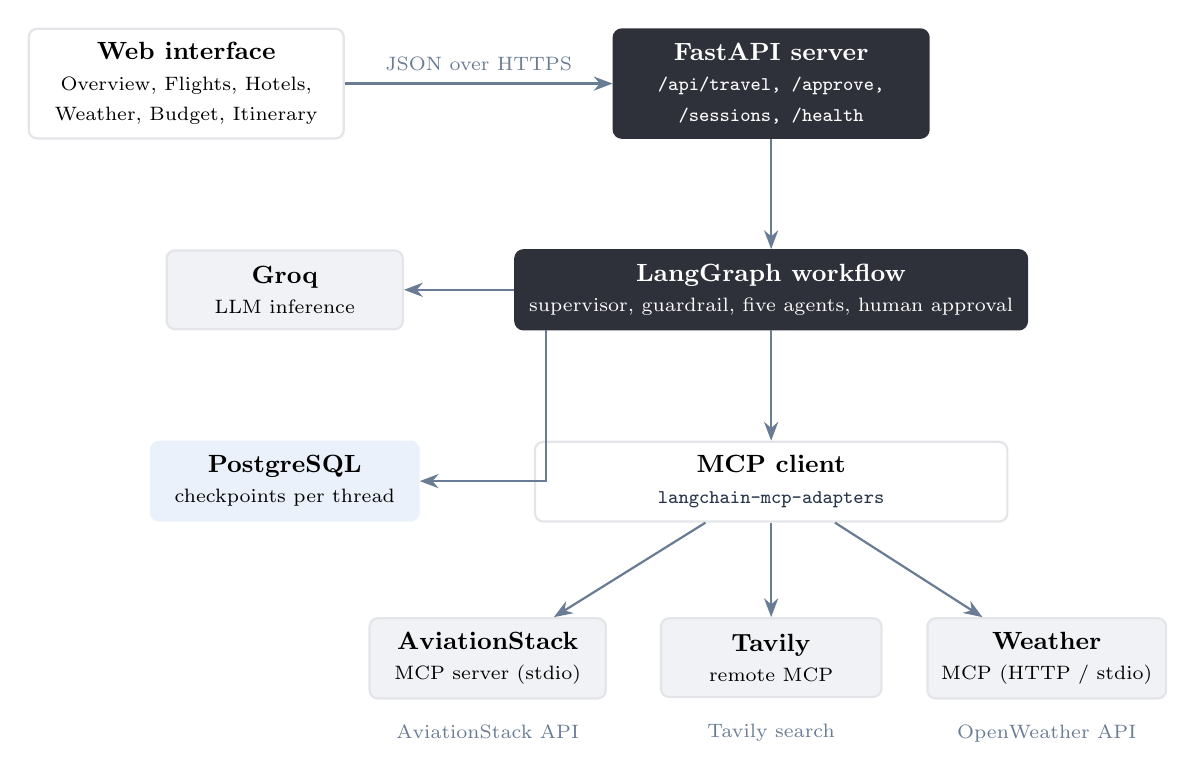
\begin{tikzpicture}[
  font=\small,
  box/.style={draw=rule,fill=white,rounded corners=3pt,align=center,minimum height=10mm,inner sep=5pt,line width=0.8pt},
  dark/.style={box,fill=ink,draw=ink,text=white},
  ext/.style={box,fill=paper},
  data/.style={box,fill=infotint,draw=infotint},
  arr/.style={-{Stealth[length=2.4mm]},line width=0.8pt,color=muted},
  lab/.style={font=\scriptsize,color=muted,fill=white,inner sep=1.5pt}]
  \node[box,minimum width=40mm] (ui) {\textbf{Web interface}\\ \scriptsize Overview, Flights, Hotels,\\ \scriptsize Weather, Budget, Itinerary};
  \node[dark,minimum width=40mm,right=34mm of ui] (api) {\textbf{FastAPI server}\\ \scriptsize\ttfamily /api/travel, /approve,\\ \scriptsize\ttfamily /sessions, /health};
  \node[dark,minimum width=60mm,below=14mm of api] (graph) {\textbf{LangGraph workflow}\\ \scriptsize supervisor, guardrail, five agents, human approval};
  \node[ext,minimum width=30mm,left=14mm of graph] (groq) {\textbf{Groq}\\ \scriptsize LLM inference};
  \node[data,minimum width=34mm,below=14mm of groq] (pg) {\textbf{PostgreSQL}\\ \scriptsize checkpoints per thread};
  \node[box,below=14mm of graph,minimum width=60mm] (mcp) {\textbf{MCP client}\\ \scriptsize \code{langchain-mcp-adapters}};
  \node[ext,below=12mm of mcp,minimum width=30mm,xshift=-36mm] (avs) {\textbf{AviationStack}\\ \scriptsize MCP server (stdio)};
  \node[ext,below=12mm of mcp,minimum width=28mm] (tav) {\textbf{Tavily}\\ \scriptsize remote MCP};
  \node[ext,below=12mm of mcp,minimum width=30mm,xshift=35mm] (wx) {\textbf{Weather}\\ \scriptsize MCP (HTTP / stdio)};
  \node[font=\scriptsize,color=muted,below=2mm of wx] {OpenWeather API};
  \node[font=\scriptsize,color=muted,below=2mm of avs] {AviationStack API};
  \node[font=\scriptsize,color=muted,below=2mm of tav] {Tavily search};
  \draw[arr] (ui) -- node[lab,above=1mm]{JSON over HTTPS} (api);
  \draw[arr] (api) -- (graph);
  \draw[arr] (graph) -- (groq);
  \draw[arr] (graph.south west) ++(4mm,0) |- (pg.east);
  \draw[arr] (graph) -- (mcp);
  \draw[arr] (mcp) -- (avs);
  \draw[arr] (mcp) -- (tav);
  \draw[arr] (mcp) -- (wx);
\end{tikzpicture}
\caption{System architecture.}\label{fig:arch}
\end{figure}

\subsection{The flow of agents}
SafrMrtah is built as a LangGraph state graph (Figure~\ref{fig:flow}). All agents share one \emph{state}: the request, the trip constraints, each agent's result, the draft itinerary and the human decision. The graph is checkpointed after each step, so a paused plan can be resumed later, even after a restart.

\begin{figure}[htbp]\centering
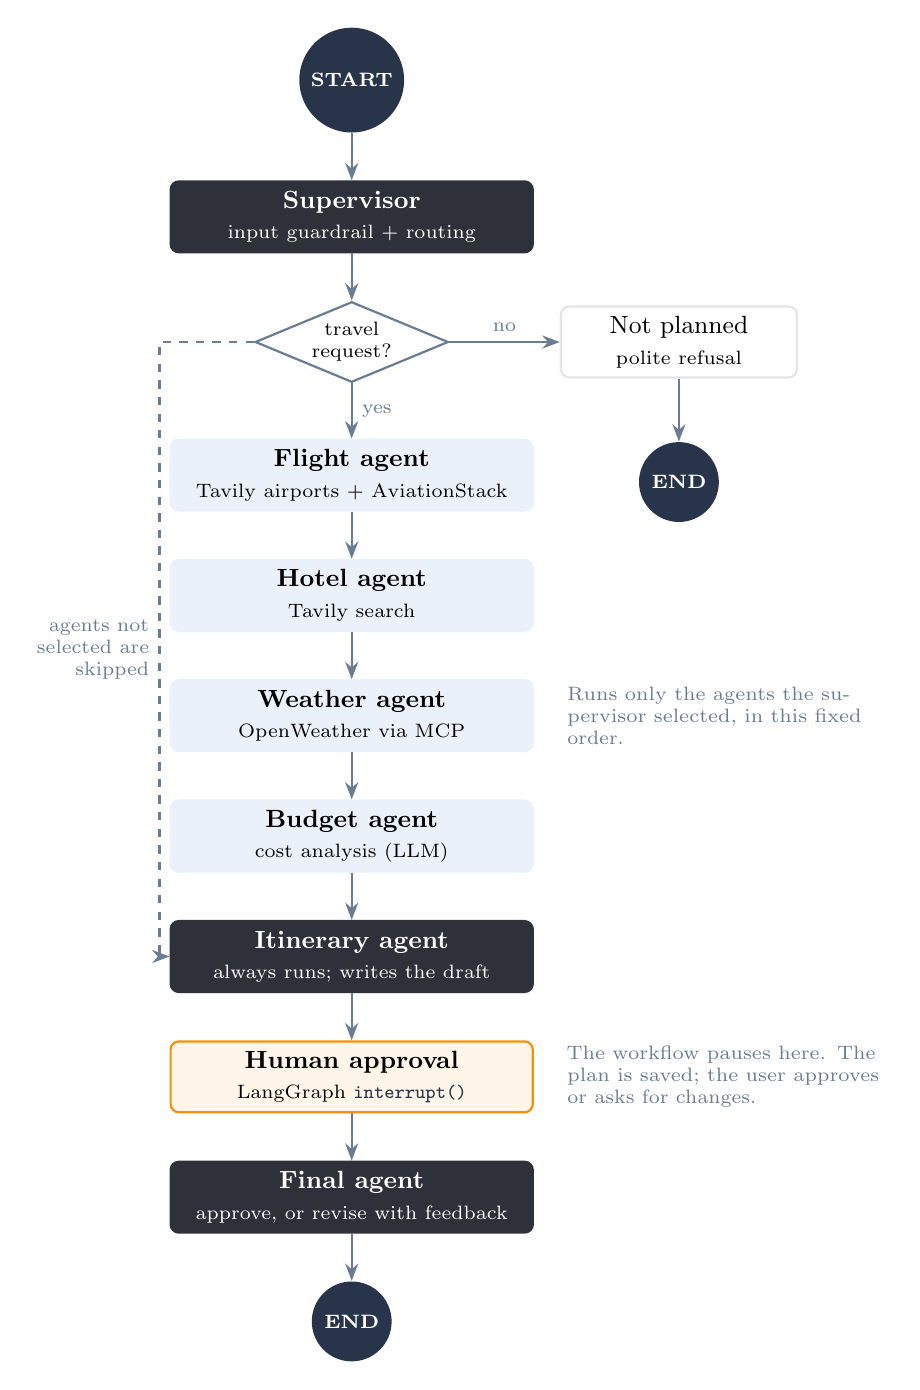
\begin{tikzpicture}[
  font=\small,
  node distance=6mm,
  stp/.style={draw=rule,fill=white,rounded corners=3pt,align=center,minimum width=46mm,minimum height=9mm,line width=0.8pt},
  agent/.style={stp,fill=infotint,draw=infotint},
  key/.style={stp,fill=ink,draw=ink,text=white},
  human/.style={stp,fill=ambertint,draw=amber},
  decision/.style={diamond,aspect=2.4,draw=muted,fill=white,align=center,inner sep=1pt,font=\scriptsize,line width=0.8pt},
  term/.style={circle,fill=slate,text=white,font=\scriptsize\bfseries,minimum size=8mm},
  arr/.style={-{Stealth[length=2.2mm]},line width=0.8pt,color=muted},
  lab/.style={font=\scriptsize,color=muted}]
  \node[term] (start) {START};
  \node[key,below=of start] (sup) {\textbf{Supervisor}\\ \scriptsize input guardrail + routing};
  \node[decision,below=of sup] (ok) {travel\\request?};
  \node[stp,right=14mm of ok,minimum width=30mm] (blocked) {Not planned\\ \scriptsize polite refusal};
  \node[agent,below=7mm of ok] (fl) {\textbf{Flight agent}\\ \scriptsize Tavily airports + AviationStack};
  \node[agent,below=of fl] (ho) {\textbf{Hotel agent}\\ \scriptsize Tavily search};
  \node[agent,below=of ho] (we) {\textbf{Weather agent}\\ \scriptsize OpenWeather via MCP};
  \node[agent,below=of we] (bu) {\textbf{Budget agent}\\ \scriptsize cost analysis (LLM)};
  \node[key,below=of bu] (it) {\textbf{Itinerary agent}\\ \scriptsize always runs; writes the draft};
  \node[human,below=of it] (hu) {\textbf{Human approval}\\ \scriptsize LangGraph \code{interrupt()}};
  \node[key,below=of hu] (fi) {\textbf{Final agent}\\ \scriptsize approve, or revise with feedback};
  \node[term,below=of fi] (end) {END};
  \node[term,below=8mm of blocked] (end2) {END};

  \draw[arr] (start) -- (sup);
  \draw[arr] (sup) -- (ok);
  \draw[arr] (ok) -- node[lab,above]{no} (blocked);
  \draw[arr] (blocked) -- (end2);
  \draw[arr] (ok) -- node[lab,right]{yes} (fl);
  \draw[arr] (fl) -- (ho); \draw[arr] (ho) -- (we); \draw[arr] (we) -- (bu); \draw[arr] (bu) -- (it);
  \draw[arr] (it) -- (hu); \draw[arr] (hu) -- (fi); \draw[arr] (fi) -- (end);

  % skip lines: agents not selected are bypassed
  \draw[arr,dashed] (ok.west) -- ++(-12mm,0) |- node[lab,pos=0.25,left,align=right]{agents not\\selected are\\skipped} (it.west);
  \node[lab,right=3mm of we,align=left,text width=40mm] {Runs only the agents the supervisor selected, in this fixed order.};
  \node[lab,right=3mm of hu,align=left,text width=40mm] {The workflow pauses here. The plan is saved; the user approves or asks for changes.};
\end{tikzpicture}
\caption{The flow of agents in the LangGraph workflow.}\label{fig:flow}
\end{figure}

\subsubsection{What each agent does}
\begin{tabularx}{\linewidth}{@{}>{\leavevmode\color{slate}\bfseries}p{30mm}L@{}}
\toprule
Supervisor & First runs the \emph{input guardrail}: an LLM check that the request is about travel and not harmful. Then it chooses the agents and extracts the trip constraints (origin, destination, duration, budget, style). The itinerary agent is always included. \\
Flight agent & Resolves the departure and arrival airport codes with Tavily, retrieves future departure and arrival schedules from AviationStack, and asks the LLM for flight guidance. It is told not to invent prices or flight numbers and to separate live data from estimates. \\
Hotel agent & Searches for hotels and areas with Tavily. \\
Weather agent & Uses the supervisor's destination to call the weather MCP server: current conditions and a daily 5-day summary. \\
Budget agent & Estimates cost categories, risks, savings and overall feasibility from the request and the other agents' results. \\
Itinerary agent & Combines everything into a draft: summary, transport, accommodation, weather, day-by-day activities, budget and tips. \\
Human approval & Pauses the graph with \code{interrupt()} and waits for the user's decision. \\
Final agent & If approved, the draft becomes the final plan. If changes were requested, the LLM revises the draft using the user's note. \\
\bottomrule
\end{tabularx}

\subsection{One request, end to end}
\begin{enumerate}[leftmargin=1.6em]
  \item The interface sends the request to \code{POST /api/travel} with a new thread.
  \item LangGraph runs the supervisor, then the selected agents, then the itinerary agent, and stops at the human-approval step. Each step is saved in PostgreSQL.
  \item The server returns the draft and every agent's result. The interface turns them into the Flights, Hotels, Weather, Budget and Itinerary pages, showing ``Not available'' for anything missing.
  \item The user approves or requests changes; \code{POST /api/travel/approve} resumes the same thread from its checkpoint and returns the final plan.
\end{enumerate}

\subsection{Interface and data handling}
The backend returns Markdown text. A normalisation layer in the browser extracts structured values conservatively: airport codes only from labelled lines, prices only when a currency is present, budget totals either as stated or clearly marked as ``added up'', and days from headings or tables. Each value carries its source. Charts were checked with a colour validator for contrast and colour-blind safety.

\subsection{API}
\begin{tabularx}{\linewidth}{@{}>{\leavevmode\color{slate}\ttfamily}p{62mm}L@{}}
\toprule
POST /api/travel & Start a plan. Body: \code{message}, optional \code{thread\_id}. \\
POST /api/travel/approve & Approve or request changes. Body: \code{thread\_id}, \code{approved}, \code{feedback}. \\
GET /api/travel/sessions & Recent trips stored in PostgreSQL. \\
GET /api/travel/session/\{id\} & One trip, rebuilt from its checkpoint. \\
GET /health & Health check; always public. \\
\bottomrule
\end{tabularx}

% =========================================================================
\section{Running and deploying}

\subsection{Configuration}
All secrets live in environment variables, never in the code or in git. \code{.env.example} lists them:

\begin{tabularx}{\linewidth}{@{}>{\leavevmode\color{slate}\ttfamily}p{56mm}L@{}}
\toprule
GROQ\_API\_KEY & Language model \\
DATABASE\_URL & PostgreSQL connection \\
TAVILY\_API\_KEY & Web search \\
AVIATIONSTACK\_API\_KEY & Flight data \\
OPENWEATHER\_API\_KEY & Weather data \\
APP\_USERNAME, APP\_PASSWORD & Sign-in for a deployed server \\
WEATHER\_MCP\_URL, WEATHER\_MCP\_TOKEN & Optional separate weather server \\
\bottomrule
\end{tabularx}

\subsection{On a Windows computer}
\begin{enumerate}[leftmargin=1.6em]
  \item Copy \code{.env.example} to \code{.env} and fill in the keys.
  \item Run \code{setup\_venv.bat} once. It creates a fresh Python environment and installs everything, including the AviationStack MCP tool.
  \item Run \code{run\_local.bat}. It starts the weather MCP server and the app; open \code{http://127.0.0.1:8000}.
\end{enumerate}
A Python environment cannot be copied between computers: on a new machine, run \code{setup\_venv.bat} again.

\subsection{Deployment on Render}
\begin{enumerate}[leftmargin=1.6em]
  \item Push the project to your own GitHub repository (\code{.env} stays local).
  \item In Render, choose \textbf{New, Blueprint}, and select the repository. Render reads \code{render.yaml} and builds the \code{Dockerfile}.
  \item Enter the API keys, the database URL and an \code{APP\_PASSWORD}.
\end{enumerate}
The container uses the port given by the host, runs as a non-root user, includes a health check, and installs the flight tool at build time. On Render's free plan the service sleeps after a period without visits and takes about a minute to wake.

\subsection{Security}
\begin{itemize}
  \item Password protection with HTTP Basic authentication when \code{APP\_PASSWORD} is set; \code{/health} stays public.
  \item Secrets are excluded from git and from the Docker image.
  \item The optional remote weather server can require a bearer token.
  \item Markdown from the AI is sanitised before it is shown, so it cannot run scripts.
  \item Everyone who has the password sees all trips: the app is designed for one person or a small team.
\end{itemize}

% =========================================================================
\section{Limitations and next steps}

\subsection{Current limitations}
\begin{itemize}
  \item Fares and costs are estimates from the language model, not bookable quotes.
  \item The weather forecast covers the next five days, not the travel dates.
  \item Flight schedules depend on the AviationStack plan; some endpoints (such as airport search) are not available on every plan, which is why airport codes are resolved with Tavily.
  \item Results depend on the quality of the language model's text; structured extraction falls back to showing the text as written.
  \item A single shared password; no individual accounts.
\end{itemize}

\subsection{Possible next steps}
\begin{itemize}
  \item User accounts, so each person sees only their own trips.
  \item Structured (JSON) output from the agents, removing the need to parse text.
  \item Live fare and hotel price APIs, and date-specific weather for the travel period.
  \item Streaming progress, so each agent's status appears as it finishes.
  \item Automated tests and evaluation of plan quality.
\end{itemize}

% =========================================================================
\clearpage
\section{Credits}
SafrMrtah is based on the open-source project \emph{Multi-Agent-System-using-LangGraph-MCP-Supervisor-Guardrails-HITL} by entbappy, released under the Apache License 2.0. This version was extended with a new interface and branding, a remote weather MCP server, session history, password protection and a deployment setup. Interface fonts: Barlow, SIL Open Font License. Icons adapted from Lucide (ISC licence).

\vspace{16mm}
\begin{center}
{\color{muted}\small Prepared by}\\[1mm]
{\heavy\large\color{slate}Mohamed Makrani}\\
{\color{accent}Data Scientist \& AI Developer}\\[2mm]
{\small\contactline}
\end{center}

\end{document}
